Luego de correr todos los experimentos notamos que la direcci\'on IP de los nodos
no necesariamente refleja su posici\'on geogr\'afica real.

Intentamos hacer uso de la herramienta www.geoiptool.com para orientarnos en
el curso de las rutas y algunas veces encontr\'abamos que no ten\'ian sentido las
ubicaciones que nos propon\'ia esta herramienta.

Un ejemplo de esto mismo seria:

~

\begin{tabular}{lll}
	\textit{\textbf{Host name}}	&	\textit{\textbf{IP}}	&	\textit{\textbf{RTT(media) ms}}	\\
	ET6-0-0-0-GRTBUECU1.red.telefonica-wholesale.net	&	94.142.103.153	&	30.104	\\
\end{tabular}

~

Dicha IP figura en geoiptool como localizada en España. Es decir que de Buenos Aires, la ruta pasar\'a por España antes de llegar a Estados Unidos,
todo con un RTT medio de 30ms. Esto no parece para nada razonable, pero el nombre del host nos presenta informaci\'on que puede contrastar aquella
prove\'ida por geoiptool. GRT\textbf{BUE}CU1 indicar\'ia que la IP realmente pertenece a Buenos Aires, algo mucho m\'as l\'ogico.

Afortunadamente capturamos los nombres de los hosts en cada salto y la mayoria tiene indicios de ubicaci\'on en sus
nombres. Claro que no siempre encontramos hosts 'bien nombrados'.

~

Otro ejemplo podr\'ia ser \emph{be2384.ccr21.\textbf{lpl}01.atlas.cogentco.com} con el c\'odigo IATA de
Liverpool.

\subsection{Moscow State University (Rusia)}

\subsubsection{Ruta}

~

\begin{tabular}{lllll}

	\textit{\textbf{Ubicaci\'on}}	&	\textit{\textbf{IP}}	&	\textit{\textbf{RTT(media) ms}}	&	\textit{\textbf{ZScore}}	&	\textit{\textbf{Tipo}}	\\
	Buenos Aires			&	200.51.240.181	&	31.018	&	0.220	&	Continental	\\
	Buenos Aires (telef\'onica)	&	94.142.103.153	&	30.104	&	-0.265	&	Continental	\\
	Miami (telef\'onica)		&	94.142.123.22	&	164.933	&	1.795	&	Trasatl\'antico	\\
	Dallas (telef\'onica)		&	94.142.127.105	&	199.813	&	0.278	&	Continental	\\
	Dallas/Ft Worth (cogentco)	&	154.54.13.225	&	221.383	&	0.077	&	Continental	\\
	Dallas/Ft Worth (cogentco)	&	154.54.7.45	&	212.266	&	-0.389	&	Continental	\\
	Kansas (cogentco)		&	154.54.2.113	&	214.954	&	-0.210	&	Continental	\\
	Chicago (cogentco)		&	154.54.6.86	&	215.663	&	-0.240	&	Continental	\\
	Toronto (cogentco)		&	154.54.27.182	&	228.466	&	-0.056	&	Continental	\\
	Montreal (cogentco)		&	154.54.30.206	&	226.107	&	-0.286	&	Continental	\\
	Liverpool (cogentco)		&	154.54.44.138	&	294.383	&	0.785	&	Continental	\\
	Amsterdam (cogentco)		&	154.54.77.245	&	307.648	&	-0.049	&	Continental	\\
	Hamburgo (cogentco)		&	154.54.74.122	&	264.320	&	-0.908	&	Continental	\\
	Estocolmo (cogentco)		&	154.54.63.2	&	327.827	&	0.713	&	Continental	\\
	Helsinki (cogentco)		&	154.54.62.250	&	332.424	&	-0.181	&	Continental	\\
	Mosc\'u				&	149.6.58.42	&	333.589	&	-0.233	&	Continental	\\
	Mosc\'u (runnet)		&	194.85.40.229	&	525.315	&	2.658	&	Trasatl\'antico	\\
	Mosc\'u (runnet)		&	194.190.254.118	&	357.420	&	-2.798	&	Continental	\\
	Mosc\'u (runnet)		&	93.180.0.172	&	344.003	&	-0.454	&	Continental	\\
	Mosc\'u				&	188.44.33.1	&	346.421	&	-0.214	&	Continental	\\
	Mosc\'u				&	188.44.50.103	&	347.007	&	-0.242	&	Continental	\\

\end{tabular}

~

Las ciudades fueron atravesadas en el siguiente orden:

Buenos Aires - Miami - Dallas - Kansas - Chicago - Toronto - Montreal - Liverpool - Amsterdam -
Hamburg - Stockolm - Helsinki - Moscow


~

\begin{figure}[H]
	\center
	\begin{subfigure}{0.4\textwidth}
		\includegraphics[width=1.0\textwidth]{../results/graficos/MSU_rtt.png}
		\caption{RTT para MSU}
	\end{subfigure}
	~
	\begin{subfigure}{0.4\textwidth}
		\includegraphics[width=1.0\textwidth]{../results/graficos/MSU_zscore.png}
		\caption{Zscore para MSU}
	\end{subfigure}
\end{figure}

~

\textcolor{red}{Podemos ver que la ruta pasa de Am\'erica del Sur (BUE) a Am\'erica del Norte (MIA), luego de Canada en America del Norte (Montreal) a Europa (Liverpool) y por \'ultimo llega a Mosk\'u en Asia. En el primero de los saltos descriptos el ZScore es bastante alto, y por eso figura como trasatl\'antico en la tabla.
Luego el segundo salto no es significativo para un umbral de 1.5, si lo ser\'a con uno de 0.5.
Dentro de los saltos en Moscu obtenemos un ZScore de 2.66 aun no siendo un enlace submarino. Esto puede deberse al entrar en la Russian University Network.}
\textcolor{blue}{ESTO AHORA HAY QUE VERLO BIEN, DEPENDE MUCHO DEL ANALISIS QUE HAGAMOS PARA EL UMBRAL, YA QUE EL TIPO SE CORRESPONDE CON ESO.}

\begin{figure}[H]
	\begin{center}
		  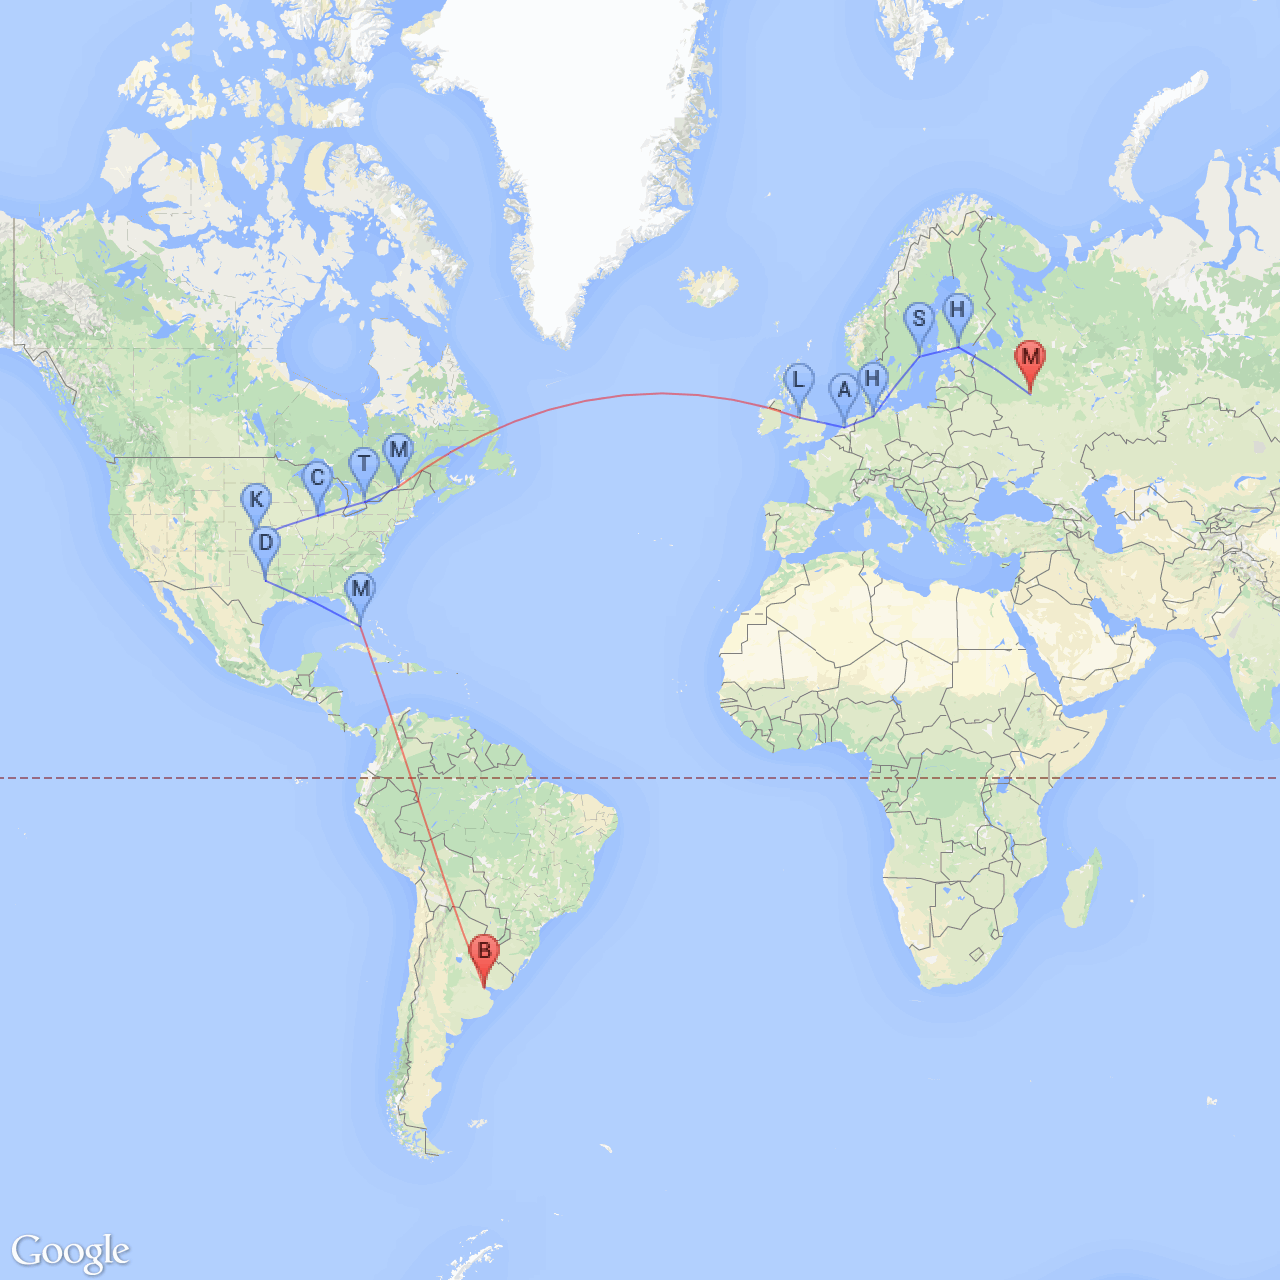
\includegraphics[scale=0.25]{../results/maps/MSU.png}
		  \caption{Mapa de la ruta atravesada para llegar a la universidad de Rusia}
	\end{center}
\end{figure}

\textcolor{red}{mas analisis y grafico de barra IP zscore + umbral}

\subsection{Tsinghua}

Para el caso de China, la ruta comienza por Estados Unidos como el caso anterior, pero en lugar de cruzar a Europa por el Este, los paquetes viajan por el pac\'ifico.
Veamos la siguiente tabla.

~

\begin{tabular}{lllll}
	\textit{\textbf{Ubicaci\'on}}	&	\textit{\textbf{IP}}	&	\textit{\textbf{RTT(media) ms}}	&	\textit{\textbf{ZScore}}	&	\textit{\textbf{Tipo}}	\\
	Buenos Aires			&	200.51.240.156	&	31.907	&	0.259	&	Continental	\\
	Buenos Aires (telef\'onica)	&	84.16.9.233	&	30.095	&	-0.437	&	Continental	\\
	Miami (telef\'onica)		&	94.142.121.222	&	165.469	&	2.396	&	Trasatl\'antico	\\
	Miami (telef\'onica)		&	94.142.122.249	&	165.140	&	-0.407	&	Continental	\\
	Miami (telef\'onica)		&	84.16.12.238	&	167.934	&	-0.342	&	Continental	\\
	Miami 				&	63.243.152.45	&	164.176	&	-0.478	&	Continental	\\
	Ashburn				&	66.198.154.177	&	265.945	&	1.702	&	Trasatl\'antico	\\
	Dallas				&	66.198.154.118	&	254.661	&	-0.633	&	Continental	\\
	Dallas				&	66.110.56.6	&	267.287	&	-0.139	&	Continental	\\
	Los-Angeles			&	66.110.57.82	&	256.103	&	-0.631	&	Continental	\\
	Los-Angeles			&	66.110.59.182	&	257.170	&	-0.378	&	Continental	\\
	Chongming				&	101.4.117.213	&	428.694	&	3.143	&	Trasatl\'antico	\\
	Chongming				&	101.4.117.97	&	428.055	&	-0.413	&	Continental	\\
	Beijing				&	101.4.116.146	&	424.990	&	-0.463	&	Continental	\\
	Beijing				&	101.4.118.78	&	427.001	&	-0.358	&	Continental	\\
	Beijing				&	202.112.38.10	&	425.663	&	-0.428	&	Continental	\\
	Beijing				&	118.229.4.66	&	425.672	&	-0.400	&	Continental	\\
	Beijing				&	118.229.4.34	&	438.217	&	-0.141	&	Continental	\\
	Beijing				&	118.229.2.74	&	430.018	&	-0.569	&	Continental	\\
	Beijing				&	118.229.2.69	&	425.922	&	-0.485	&	Continental	\\
	Beijing				&	118.229.8.6	&	427.147	&	-0.375	&	Continental	\\
	Beijing (Tsinghua)		&	166.111.4.100	&	426.084	&	-0.422	&	Continental	\\

\end{tabular}

~

Las ciudades fueron atravesadas en el siguiente orden:

Buenos Aires - Miami - Ashburn - Dallas - Los \'Angeles - Chongming - Beijing

~

\begin{figure}[H]
	\center
	\begin{subfigure}{0.4\textwidth}
		\includegraphics[width=1.0\textwidth]{../results/graficos/Tsinghua_rtt.png}
		\caption{RTT para Tsinghua}
	\end{subfigure}
	~
	\begin{subfigure}{0.4\textwidth}
		\includegraphics[width=1.0\textwidth]{../results/graficos/Tsinghua_zscore.png}
		\caption{Zscore para Tsinghua}
	\end{subfigure}
\end{figure}

~


Podemos destacar tres enlaces que superan el umbral de 1.5. Buenos Aires $\rightarrow$ Miami; Miami $\rightarrow$ Ashburn y Los-Angeles $\rightarrow$ Beijing.
De estos tres, el m\'as preocupante es el segundo, puesto que es un enlace continental, dentro de Estados Unidos.

\begin{figure}[H]
	\begin{center}
		  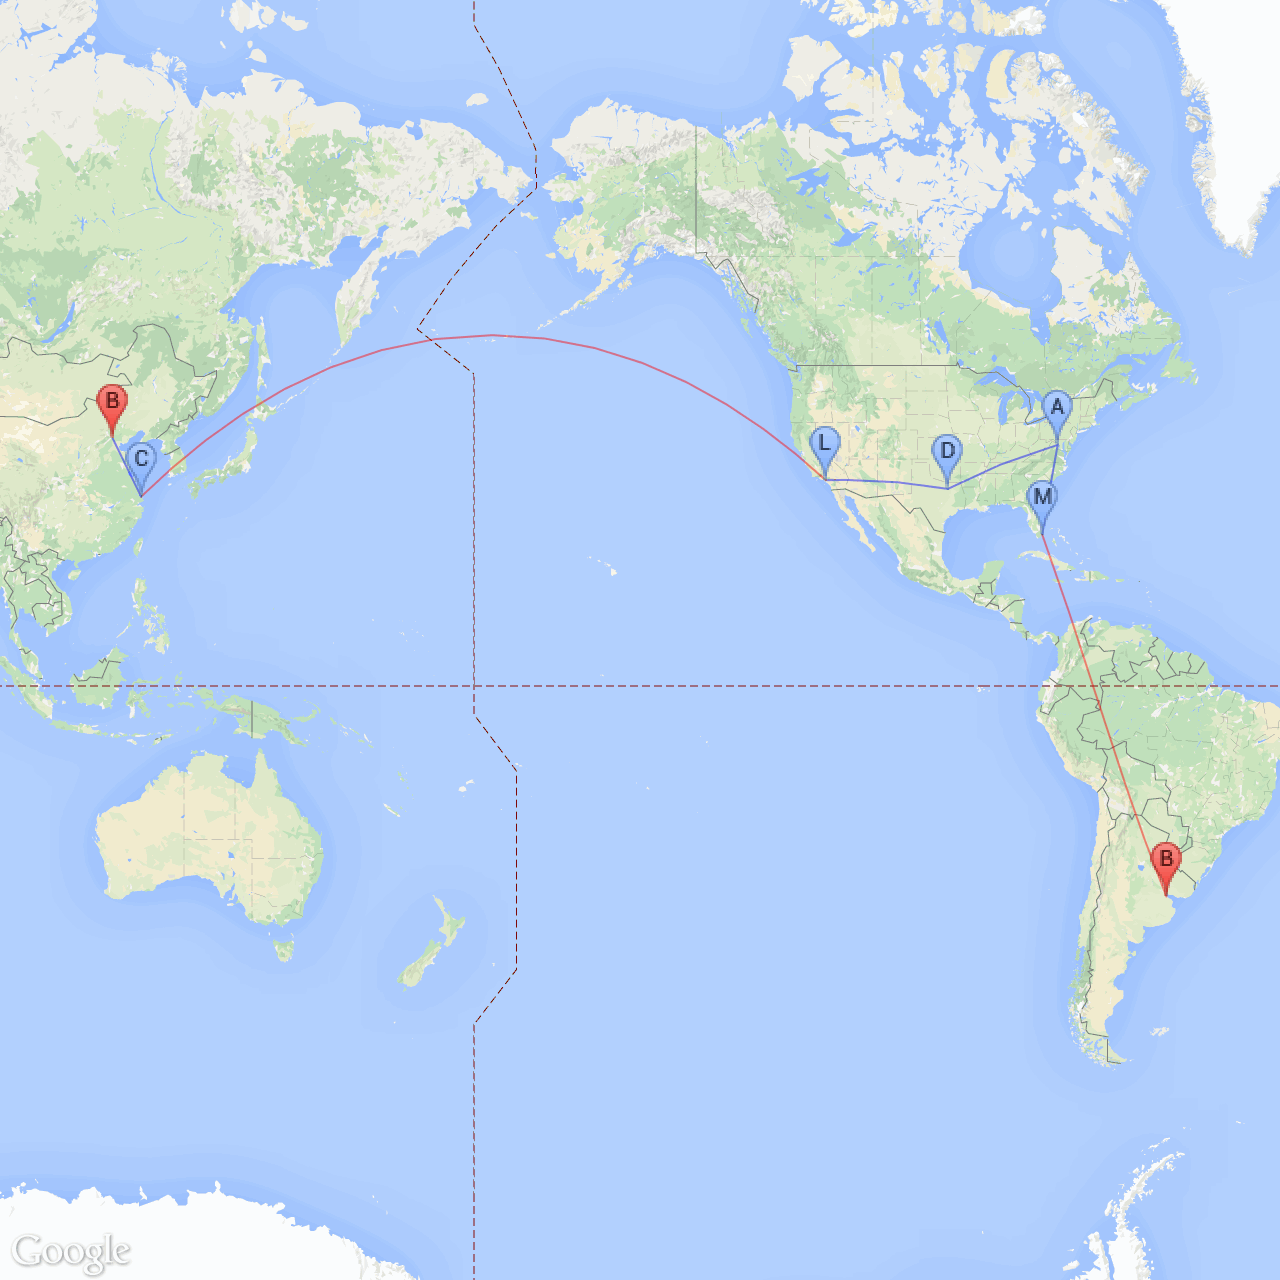
\includegraphics[scale=0.25]{../results/maps/Tsinghua.png}
		  \caption{Mapa de la ruta atravesada para llegar a la universidad de China}
	\end{center}
\end{figure}

\textcolor{red}{mas analisis y grafico de barra IP zscore + umbral}

\subsection{Oxford}

~

\begin{tabular}{lllll}
	\textit{\textbf{Ubicaci\'on}}	&	\textit{\textbf{IP}}	&	\textit{\textbf{RTT(media) ms}}	&	\textit{\textbf{ZScore}}	&	\textit{\textbf{Tipo}}	\\
	Buenos Aires			&	200.51.240.181	&	37.154	&	0.426	&	Continental	\\
	Buenos Aires (telef\'onica)	&	84.16.9.233	&	51.008	&	-0.009	&	Continental	\\
	Miami (telef\'onica)		&	5.53.5.138	&	210.915	&	2.722	&	Trasatl\'antico	\\
	Miami (telef\'onica)		&	94.142.123.5	&	174.734	&	-0.945	&	Continental	\\
	Miami (as6453)			&	63.243.152.45	&	175.240	&	-0.259	&	Continental	\\
	Ashburn (as6453)		&	66.198.154.177	&	293.857	&	1.950	&	Trasatl\'antico	\\
	Ashburn (as6453)		&	216.6.87.1	&	286.600	&	-0.404	&	Continental	\\
	Newark (as6453)			&	216.6.87.138	&	277.667	&	-0.435	&	Continental	\\
	Newark (as6453)			&	66.198.70.1	&	307.315	&	0.286	&	Continental	\\
	Londres (as6453)		&	66.198.70.26	&	403.133	&	1.523	&	Trasatl\'antico	\\
	Londres (as6453)		&	80.231.130.42	&	298.757	&	-2.220	&	Continental	\\
	195.219.100.82			&	195.219.100.82	&	285.687	&	-0.513	&	Continental	\\
	Londres				&	146.97.33.2	&	289.063	&	-0.205	&	Continental	\\
	Londres				&	146.97.37.206	&	291.484	&	-0.223	&	Continental	\\
	Londres				&	193.63.108.129	&	281.783	&	-0.450	&	Continental	\\
	Londres				&	193.63.108.134	&	294.226	&	-0.036	&	Continental	\\
	Londres				&	193.63.109.114	&	289.814	&	-0.351	&	Continental	\\
	Londres				&	192.76.21.21	&	280.879	&	-0.435	&	Continental	\\
	Londres				&	192.76.22.201	&	282.251	&	-0.243	&	Continental	\\
	Londres				&	192.76.32.66	&	286.466	&	-0.190	&	Continental	\\
	Londres				&	129.67.242.155	&	301.388	&	0.011	&	Continental	\\

\end{tabular}

~

Las ciudades fueron atravesadas en el siguiente orden:

Buenos Aires - Miami - Ashburn - Newark - London - Oxford

~

\begin{figure}[H]
	\center
	\begin{subfigure}{0.4\textwidth}
		\includegraphics[width=1.0\textwidth]{../results/graficos/Oxford_rtt.png}
		\caption{RTT para Oxford}
	\end{subfigure}
	~
	\begin{subfigure}{0.4\textwidth}
		\includegraphics[width=1.0\textwidth]{../results/graficos/Oxford_zscore.png}
		\caption{Zscore para Oxford}
	\end{subfigure}
\end{figure}

~

En este caso destacamos nuevamente tres enlaces que superan el umbral de 1.5. Buenos Aires $\rightarrow$ Miami; Miami $\rightarrow$ Ashburn y Newark $\rightarrow$ Londres.
Los dos primeros son identicos al caso anterior, nuevamente preocupa el segundo por las mismas razones.

\begin{figure}[H]
	\begin{center}
		  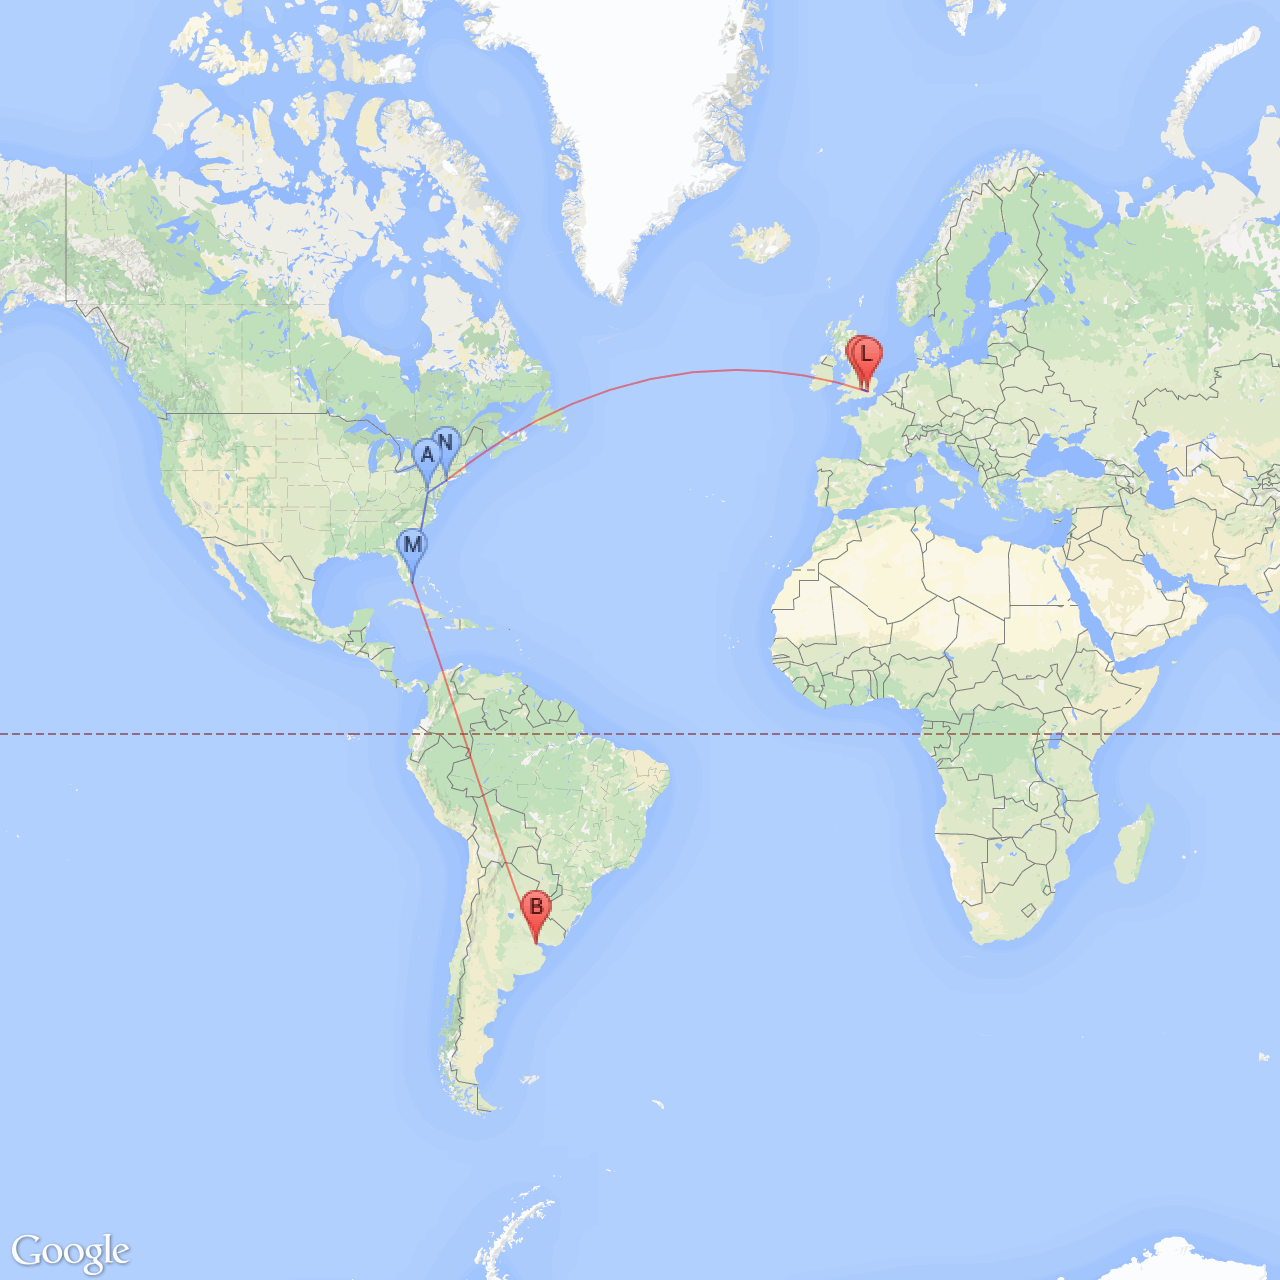
\includegraphics[scale=0.25]{../results/maps/Oxford.png}
		  \caption{Mapa de la ruta atravesada para llegar a la universidad de Inglaterra}
	\end{center}
\end{figure}

\textcolor{red}{mas analisis y grafico de barra IP zscore + umbral}

\subsection{Queensland}

~

\begin{tabular}{lllll}
	\textit{\textbf{Ubicaci\'on}}	&	\textit{\textbf{IP}}	&	\textit{\textbf{RTT(media) ms}}	&	\textit{\textbf{ZScore}}	&	\textit{\textbf{Tipo}}	\\
	Buenos Aires			&	200.51.240.156	&	31.896	&	0.110	&	Continental	\\
	Buenos Aires (telef\'onica)	&	84.16.9.233	&	30.748	&	-0.399	&	Continental	\\
	Miami (telef\'onica)		&	94.142.123.14	&	165.811	&	1.700	&	Trasatl\'antico	\\
	213.140.49.13			&	213.140.49.13	&	230.069	&	0.609	&	Continental	\\
	xe-3-1-1.mpr1.pao1.us.above.net	&	64.125.13.113	&	229.511	&	-0.390	&	Continental	\\
	208.185.52.74			&	208.185.52.74	&	392.486	&	2.131	&	Trasatl\'antico	\\
	xe-1-2-1.pe2.brwy.nsw.aarnet.net.au		&	202.158.194.176	&	391.129	&	-0.403	&	Continental	\\
	Sydney (aarnet)			&	113.197.15.57	&	514.913	&	1.527	&	Trasatl\'antico	\\
	Brisbane (aarnet)		&	202.158.194.54	&	407.555	&	-2.037	&	Continental	\\
	Brisbane (aarnet)		&	202.158.194.213	&	394.376	&	-0.585	&	Continental	\\
	Queensland (aarnet)		&	202.158.209.3	&	394.951	&	-0.373	&	Continental	\\
	Queensland (aarnet)		&	113.197.8.34	&	391.479	&	-0.435	&	Continental	\\
	Queensland			&	130.102.159.1	&	392.041	&	-0.373	&	Continental	\\
	Queensland			&	130.102.0.242	&	401.994	&	-0.228	&	Continental	\\
	Queensland			&	130.102.82.28	&	403.280	&	-0.362	&	Continental	\\
	Queensland			&	130.102.131.70	&	396.128	&	-0.492	&	Continental	\\
\end{tabular}

~

Las ciudades fueron atravesadas en el siguiente orden:

Buenos Aires - Miami - Hermosa Beach - Sydney - Brisbane - Queensland

~

\begin{figure}[H]
	\center
	\begin{subfigure}{0.4\textwidth}
		\includegraphics[width=1.0\textwidth]{../results/graficos/Queensland_rtt.png}
		\caption{RTT para Queensland}
	\end{subfigure}
	~
	\begin{subfigure}{0.4\textwidth}
		\includegraphics[width=1.0\textwidth]{../results/graficos/Queensland_zscore.png}
		\caption{Zscore para Queensland}
	\end{subfigure}
\end{figure}

~



\begin{figure}[H]
	\begin{center}
		  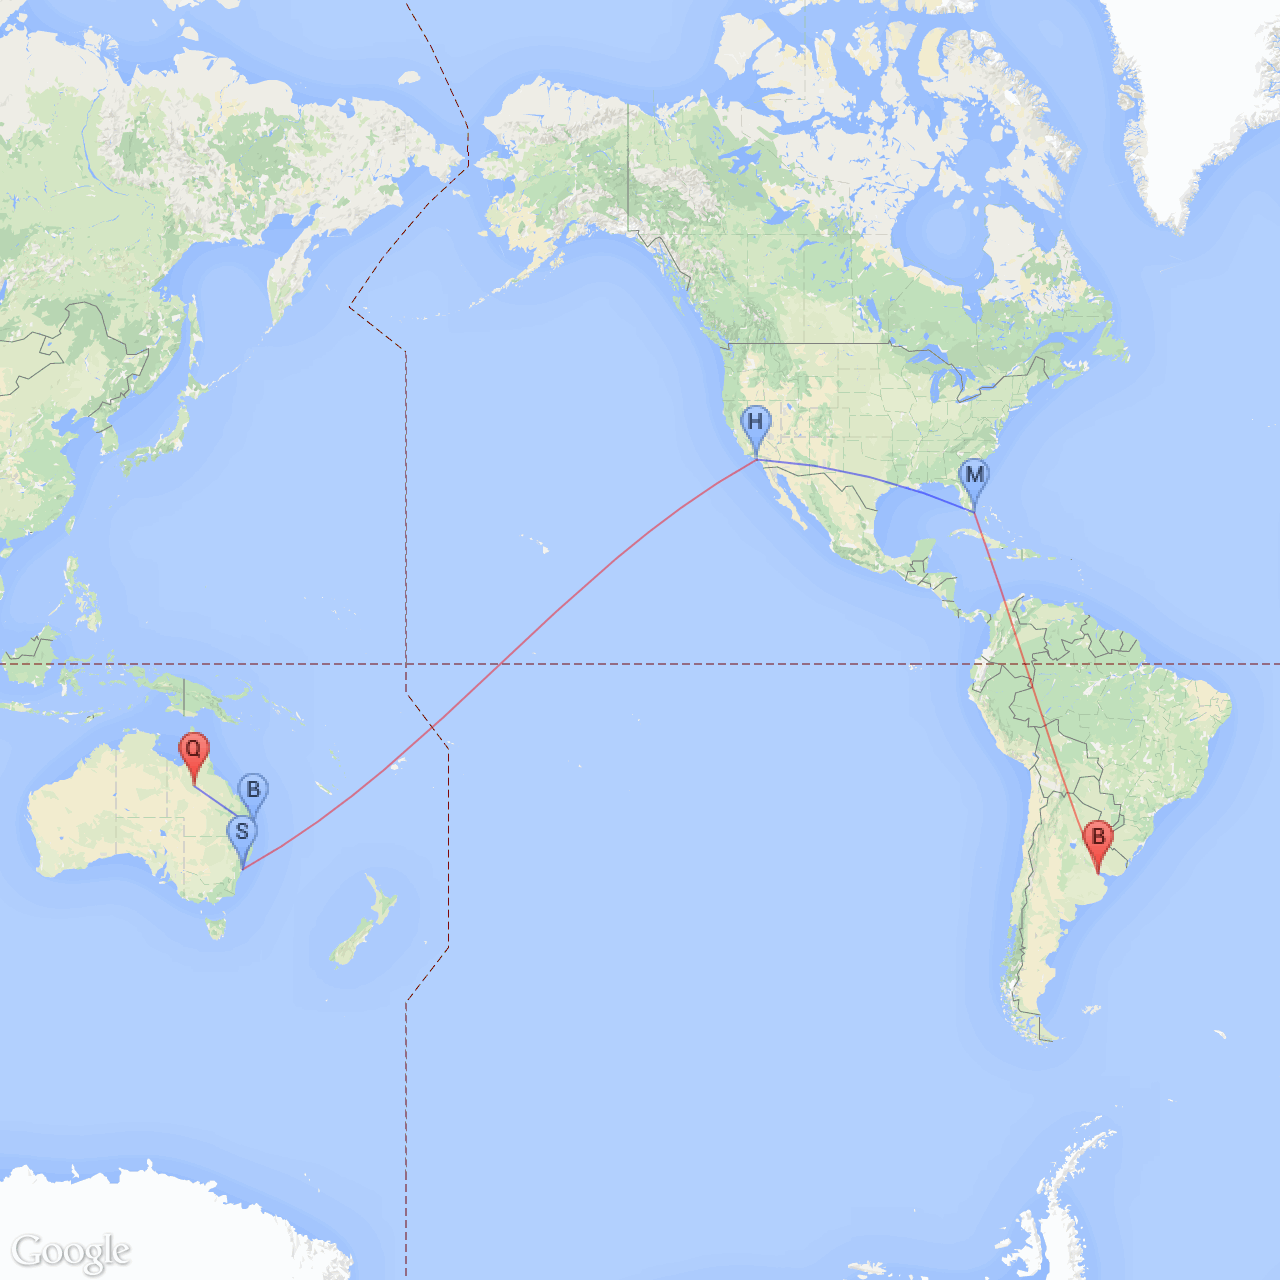
\includegraphics[scale=0.25]{../results/maps/Queensland.png}
		  \caption{Mapa de la ruta atravesada para llegar a la universidad de Australia}
	\end{center}
\end{figure}

\textcolor{red}{mas analisis y grafico de barra IP zscore + umbral}
